\documentclass[aspectratio=169, 11pt]{beamer}

\usepackage[T1]{fontenc}
\usepackage[utf8]{inputenc}
\usepackage{graphicx}
\usepackage{xcolor}
\usepackage{booktabs}

% ── Colours ──────────────────────────────────────────────────────────────────
\definecolor{darkblue}{HTML}{284b63}
\definecolor{appblue}{HTML}{2f80ed}
\definecolor{apporange}{HTML}{f2a93b}
\definecolor{appred}{HTML}{c0392b}
\definecolor{lightgray}{HTML}{f5f5f5}

% ── Theme — clean white, minimal ─────────────────────────────────────────────
\usetheme{default}
\setbeamercolor{frametitle}{fg=black}
\setbeamercolor{normal text}{fg=black}
\setbeamercolor{structure}{fg=darkblue}
\setbeamercolor{itemize item}{fg=darkblue}
\setbeamercolor{itemize subitem}{fg=darkblue}
\setbeamercolor{enumerate item}{fg=darkblue}

\setbeamerfont{frametitle}{size=\Large, series=\bfseries}
\setbeamerfont{title}{size=\huge, series=\bfseries}

\setbeamertemplate{navigation symbols}{}
\setbeamertemplate{itemize item}{$\bullet$}
\setbeamertemplate{itemize subitem}{--}
\setbeamertemplate{footline}{%
  \hfill\footnotesize\color{gray}\insertframenumber\hspace{6pt}\vspace{4pt}%
}

% ── Helpers ──────────────────────────────────────────────────────────────────
\newcommand{\tuplerow}[2]{%
  \textbf{#1}\,: \textit{#2}\\[1pt]%
}

\begin{document}

% ────────────────────────────────────────────────────────────────────────────
%  SLIDE 1 — Intro
% ────────────────────────────────────────────────────────────────────────────
\begin{frame}[t]{}
\vspace{-2pt}
{\LARGE\bfseries Visual Analytics: Project 1}

\vspace{4pt}
{\large\color{darkblue}Board Game Analysis}

\vspace{8pt}
\textbf{Task 2.1:} Explore how maximum playtime relates to ratings and review counts across board games\\[3pt]
\textbf{Task 2.2:} Compare rank-based groups using LDA dimensionality reduction

\vspace{8pt}
\begin{columns}[T]
\column{0.48\textwidth}
  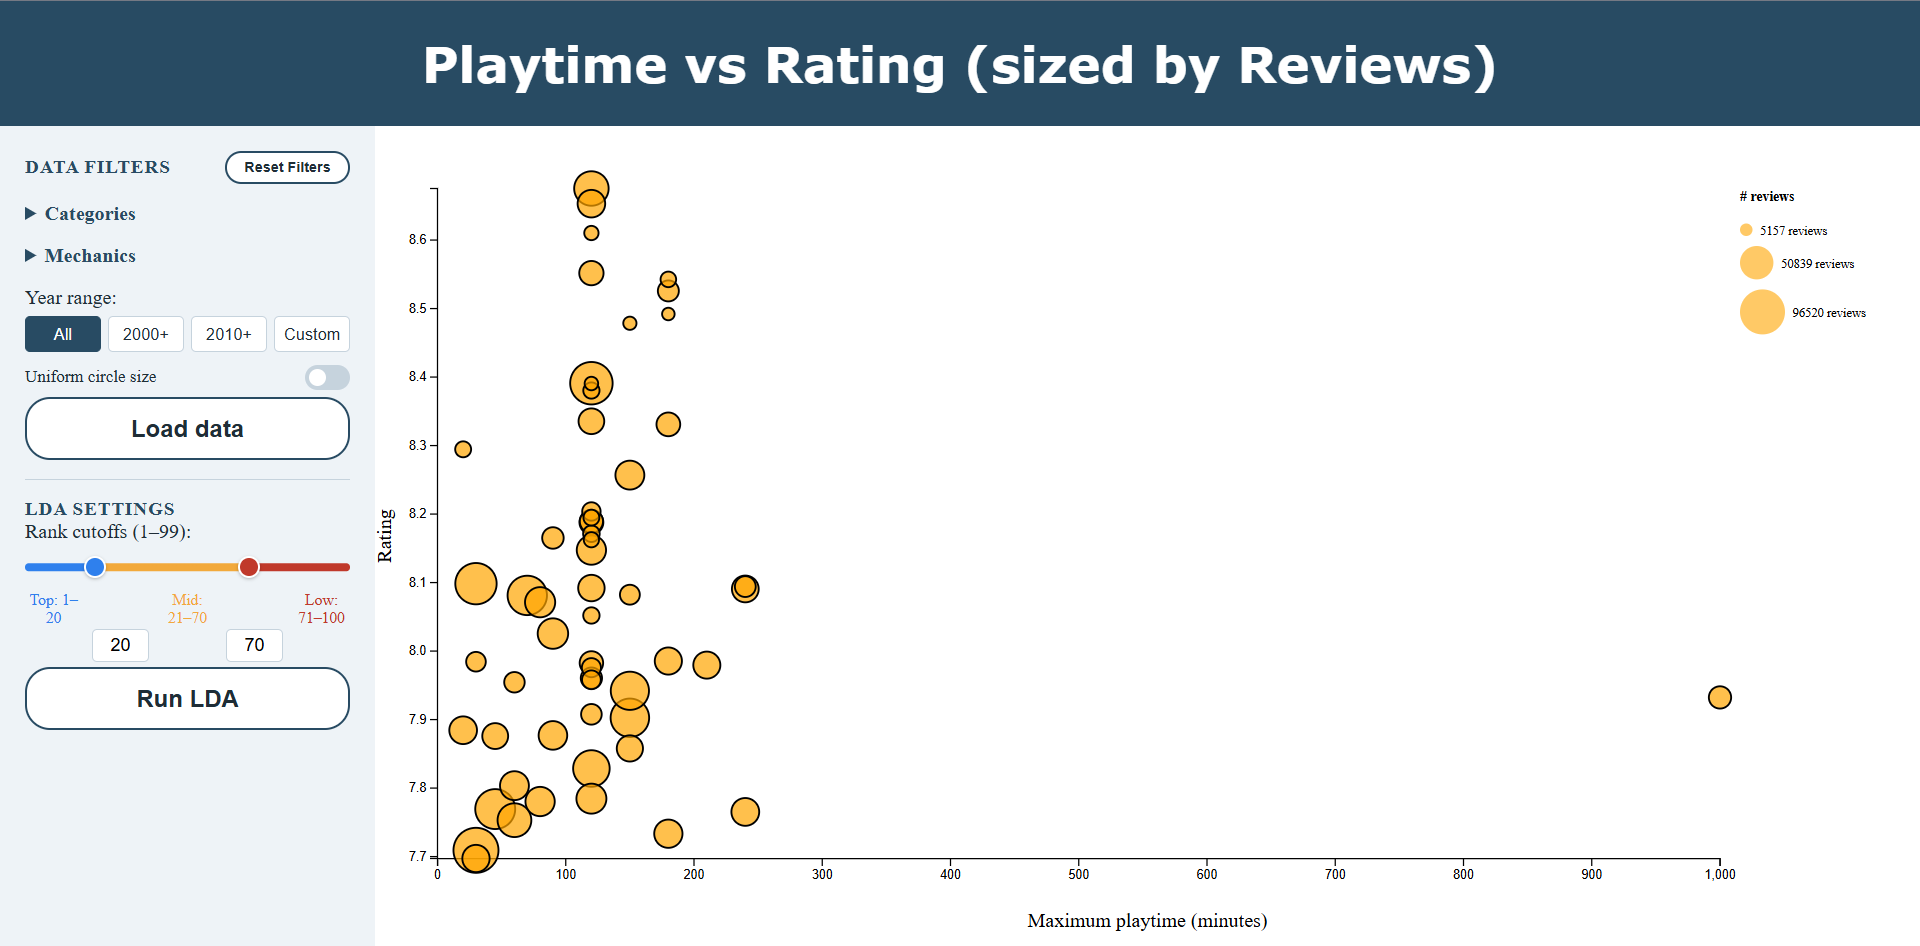
\includegraphics[width=\linewidth, height=0.42\textheight, keepaspectratio]{task21.png}

\column{0.48\textwidth}
  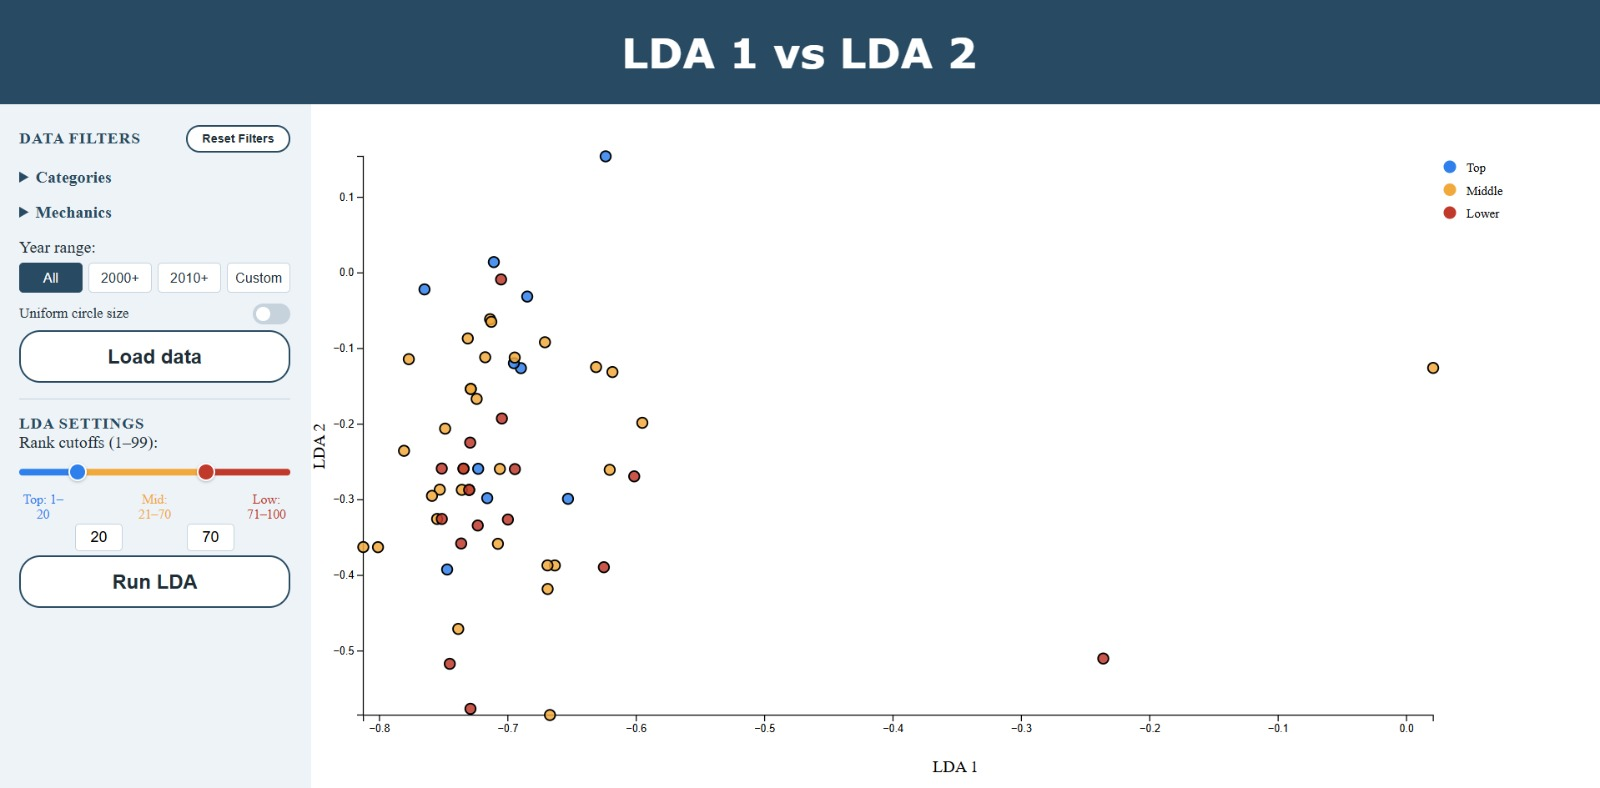
\includegraphics[width=\linewidth, height=0.42\textheight, keepaspectratio]{task22.jpeg}
\end{columns}

\vspace{6pt}
\footnotesize
\begin{columns}[T]
\column{0.48\textwidth}
\textbf{Yeganeh:} Brainstorming (5\,h), Scatterplot, LDA, year filter, rank slider, most visual design (40\,h)\\[4pt]
\textbf{G\"{o}rkem:} Brainstorming (5\,h), Category \& Mechanics filter

\column{0.48\textwidth}
\textbf{Gaurav:} Brainstorming (5\,h), Auto-refresh LDA and zoom-in (5\,h), Editing presentation (5\,h)\\[4pt]
\textbf{Hassan:} Brainstorming (5\,h)
\end{columns}
\end{frame}

% ────────────────────────────────────────────────────────────────────────────
%  SLIDE 2 — Why these tasks?
% ────────────────────────────────────────────────────────────────────────────
\begin{frame}[t]{Why these tasks?}

\begin{columns}[T]
\column{0.54\textwidth}
  \begin{itemize}\setlength\itemsep{6pt}
    \item \textbf{Task 2.1 (Explore / Correlate):}\\
          ``Does maximum playtime predict rating and commercial reach?''\\
          \textcolor{darkblue}{$\hookrightarrow$} A developer planning game length needs to know if longer games score higher and reach more players.

    \item \textbf{Task 2.2 (Compare / Group):}\\
          ``Do top-ranked games have systematically different design characteristics?''\\
          \textcolor{darkblue}{$\hookrightarrow$} If top-ranked games, cluster separately, there is a learnable design profile useful for a game developer.
  \end{itemize}

\column{0.42\textwidth}
  \small
  \vspace{2pt}
  \textbf{Task 2.1 - 5-tuple}\\[2pt]
  \tuplerow{Goal}{Explore}
  \tuplerow{Means}{Identify}
  \tuplerow{Characteristics}{Correlate}
  \tuplerow{Target}{maxplaytime , rating , num\_of\_reviews}
  \tuplerow{Cardinality}{Overall}

  \vspace{8pt}
  \textbf{Task 2.2 - 5-tuple}\\[2pt]
  \tuplerow{Goal}{Explore}
  \tuplerow{Means}{Compare}
  \tuplerow{Characteristics}{Group}
  \tuplerow{Target}{year , minage , minplayers, maxplayers, minplaytime, maxplaytime}
  \tuplerow{Cardinality}{Overall}
\end{columns}

\end{frame}

\begin{frame}[t]{Task 2.1: Playtime vs.\ Rating}

\begin{columns}[T]
\column{0.52\textwidth}
  \vspace*{40pt}
  \centering
  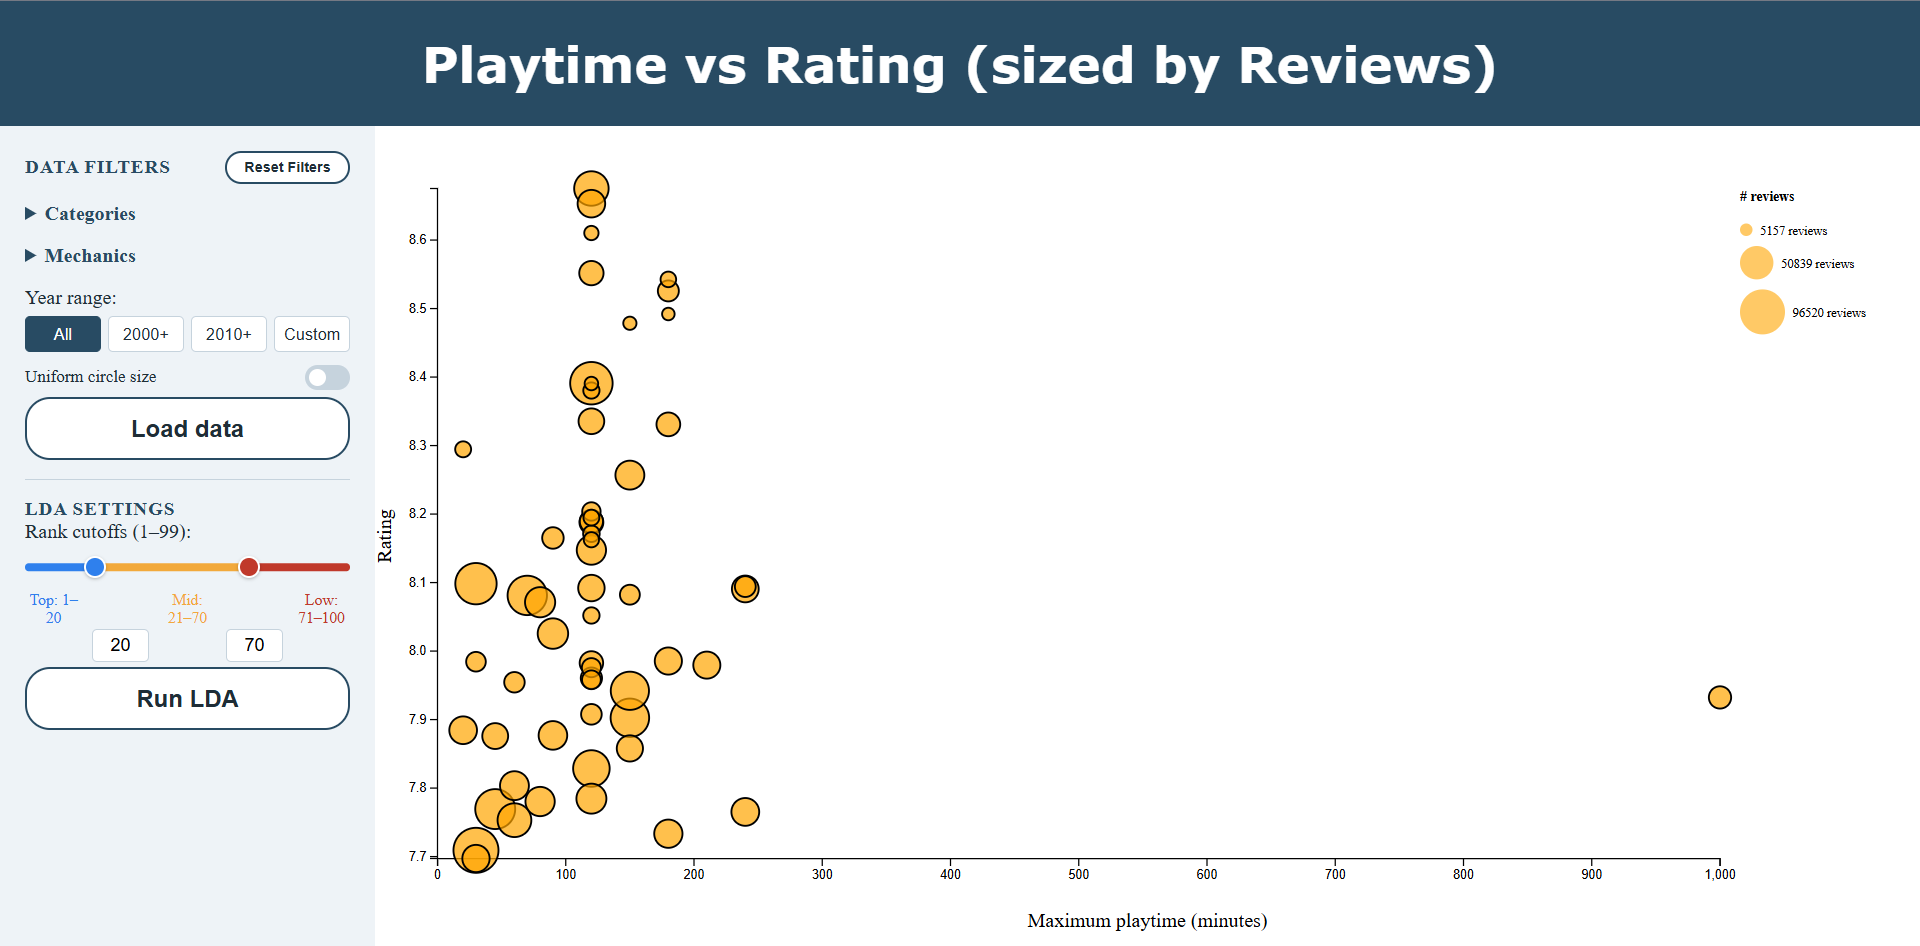
\includegraphics[width=\linewidth]{task21.png}

\column{0.45\textwidth}
  \vspace*{10pt}
  \textbf{Visualization:} Scatterplot

  \vspace{10pt}
  \begin{tabular}{@{}p{0.22\linewidth}p{0.72\linewidth}@{}}
    x-axis   & Maximum playtime (min) \\
    y-axis   & Rating \small(\texttt{d3.extent}) \\
    circle r & \# reviews \small(\texttt{scaleSqrt}) \\
    colour   & Orange (uniform) \\
  \end{tabular}

  \vspace{14pt}
  \textbf{Preprocessing:}

  \vspace{4pt}
  Nested JSON $\to$ flat object: \\
  \small\texttt{\{title, maxplaytime, rating,} \\
  \texttt{num\_of\_reviews\}}

  \vspace{14pt}
  \textbf{Included:} size legend, tooltip \\
  \textbf{Excluded:} colour groups, grid lines
\end{columns}

\end{frame}

\begin{frame}[t]{Task 2.1: Why this visualization supports the task}

\begin{itemize}\setlength\itemsep{8pt}
  \item \textbf{Scatterplot for Correlate:} Position is the most accurate visual representation for two quantitative attributes. A visible trend or spread in the point cloud directly answers the \textit{Correlate} characteristic.

  \item \textbf{\texttt{scaleSqrt} for circle size:} We perceive area, not radius. A linear radius scale makes a 4x data value appear 16x visually. \texttt{scaleSqrt} makes area grow linearly, a more accurate encoding of review count.

  \item \textbf{\texttt{d3.extent} for y-axis:} Ratings span only 7.7--8.7. Starting at 0 compresses all variation into the top 10\% of the chart.

  \item \textbf{No colour in Task 2.1:} There are no groups to distinguish. Colour here would imply conclusions that do not exist.

  \item \textbf{No grid lines:} The task is pattern detection, not precise reading. Grid lines add clutter without helping \textit{Correlate}.
\end{itemize}

\end{frame}

\begin{frame}[t]{Task 2.2: Rank Groups}

\begin{columns}[T]
\column{0.52\textwidth}
  \vspace*{40pt}
  \centering
  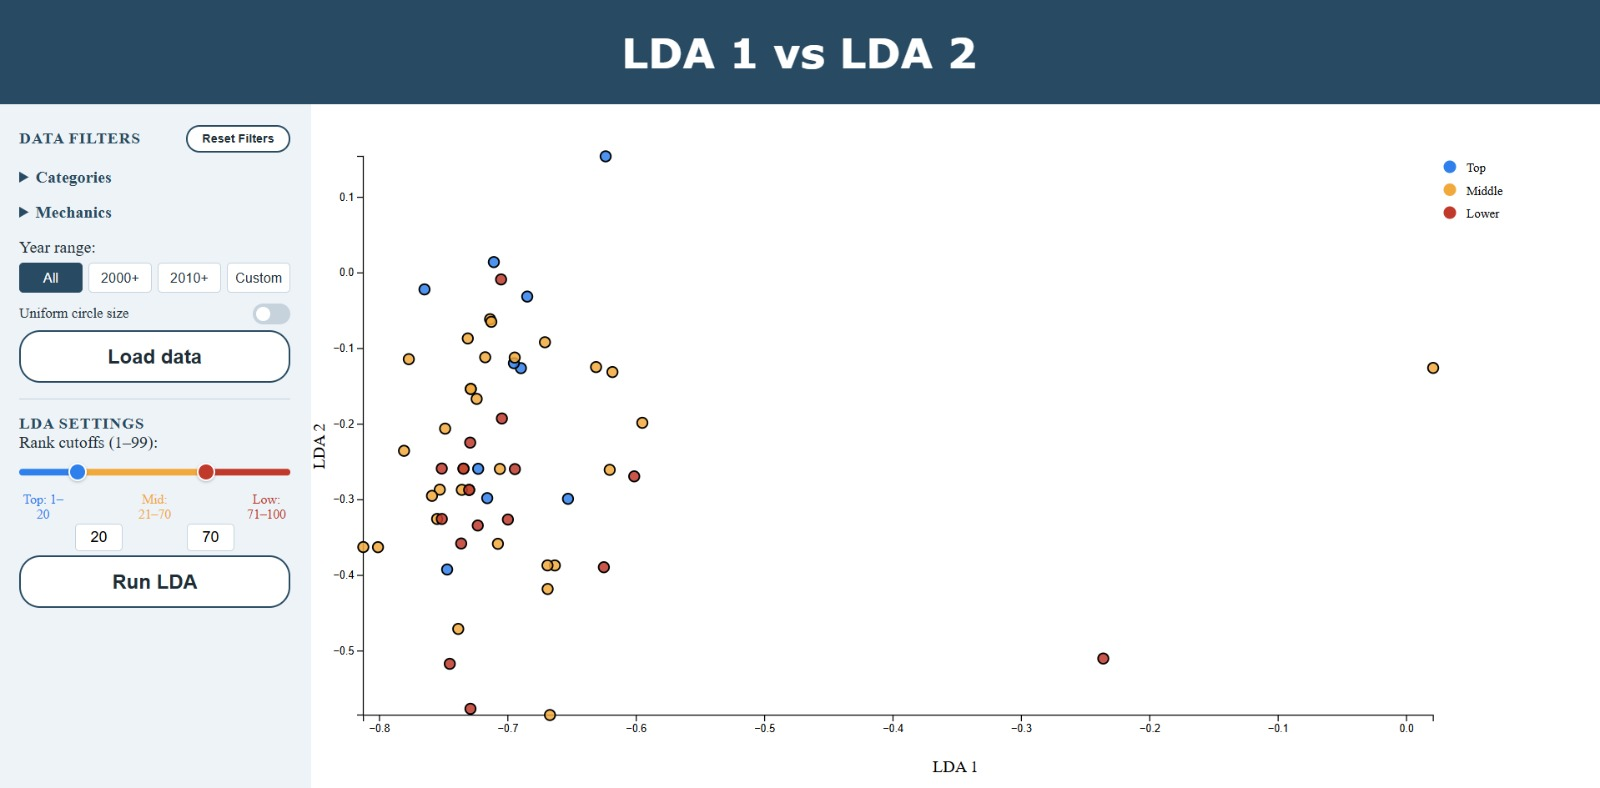
\includegraphics[width=\linewidth]{task22.jpeg}

\column{0.45\textwidth}
  \vspace{4pt}
  \textbf{Visualization:} LDA Scatterplot

  \vspace{8pt}
  \begin{tabular}{ll}
    x-axis   & LDA 1\\
    y-axis   & LDA 2\\
    colour   & Rank group\\
  \end{tabular}

  \vspace{6pt}
  \textcolor{appblue}{$\bullet$} Top (1--25)\quad
  \textcolor{apporange}{$\bullet$} Mid (26--75)\quad
  \textcolor{appred}{$\bullet$} Lower (76--100)


  \vspace{10pt}
  \textbf{LDA features} (normalised to [0,1]):\\
  \small year, minage, minplayers, maxplayers,\\
  minplaytime, maxplaytime

  \vspace{8pt}
  \textbf{\color{appred}Excluded:} \small rating, num\_of\_reviews\\
  Rank is derived from these, including them is circular reasoning.
\end{columns}

\end{frame}

\begin{frame}[t]{Task 2.2: Why this visualization supports the task}

\begin{itemize}\setlength\itemsep{8pt}
  \item \textbf{LDA for Compare + Group:} LDA is supervised, which means it finds the projection that \textit{maximally separates} labelled groups. PCA would not guarantee group separation.

  \item \textbf{Feature normalisation:} \texttt{year} ($\approx$2010) vs.\ \texttt{minplayers} ($\approx$2) differ by 1000x. Without normalisation LDA is dominated by year. All features scaled to [0,\,1].

  \item \textbf{Colour legend included:} Without it, the three groups are unidentifiable.

  \item \textbf{Tooltip included:} There are overlapping circles; without it no individual game can be named.

  \item \textbf{Variable circle size excluded:} No meaningful 3rd attribute in this view. Variable size would add noise without encoding anything real.
\end{itemize}

\end{frame}

\begin{frame}[t]{Task 2.3: Interacting with LDA Parameters}

\footnotesize
\begin{columns}[T]
\column{0.56\textwidth}
  \textbf{Interactions implemented:}
  \begin{enumerate}\setlength\itemsep{4pt}
    \item \textbf{Dual-handle rank cutoff slider}\\
          Colour-coded track (blue/orange/red). Text inputs allow precise entry. Labels show exact ranges in real time. After entering the LDA view once, slider changes refresh the projection automatically.

    \item \textbf{Year range preset buttons}\\
          All / 2000+ / 2010+ / Custom.\\
          98 of 100 games are from 2002--2021, so a continuous slider over 145 years (Crokinole, 1876) would be awkward.

    \item \textbf{Category \& Mechanics filters}\\
          Checkbox lists with live search, applied server-side before preprocessing.

    \item \textbf{Rectangular zoom-in}\\
          Drag over a crowded region to zoom into that area. Double-click restores the full view.
  \end{enumerate}

\column{0.40\textwidth}
  \textbf{Why low interaction cost?}
  \begin{itemize}\setlength\itemsep{3pt}
    \item Slider drag \textbf{or} text field to set cutoffs
    \item One initial click: \textbf{Run LDA}
    \item Later slider changes update automatically
    \item Result updates in the same view with no need for reload
  \end{itemize}

  \vspace{4pt}
  \textbf{Why rank cutoff is the key parameter:}\\
  LDA is supervised, i.e, class labels are its most important input. Changing them redefines what ``top'' means. Top~$\leq$~10 asks a different question than Top~$\leq$~50.
\end{columns}


\end{frame}

\begin{frame}[t]{Demo}

\vspace{30pt}
\centering
{\large\texttt{http://localhost:3231}}

\vspace{24pt}
\begin{enumerate}\large\setlength\itemsep{10pt}
  \item \textbf{Load data} $\to$ explore scatterplot, hover over circles
  \item \textbf{Run LDA} with default cutoffs (25 / 75)
  \item \textbf{Adjust rank cutoffs} $\to$ see LDA change actively
  \item \textbf{Filter by year} (2010+) $\to$ Load data $\to$ Run LDA
\end{enumerate}

\end{frame}

\begin{frame}[t]{What could be improved?}

\begin{itemize}\setlength\itemsep{10pt}
  \item \textbf{Task 2.1:}\\
        Brushing \& linking - selecting games in the scatterplot highlights them in the LDA view, connecting both analyses.

  \item \textbf{Task 2.2:}\\
        LDA feature importance - show which of the 6 features contribute most to LDA 1 and LDA 2, making the axes interpretable.\\[4pt]
        Game mechanics as LDA features, one-hot encoding of mechanics could better explain rank differences than design parameters alone.

  \item \textbf{General:}\\
        Richer tooltip - add mechanics, categories, and player count so the viewer can explain why a game sits where it does.\\[4pt]
        Larger dataset - all 100 games are already top-100 BGG, so there is no ``bad game'' baseline for comparison.
\end{itemize}

\end{frame}

\end{document}
